\documentclass[10pt]{beamer}
%\documentclass[10pt,handout]{beamer}
\usepackage[english]{babel}
% % \usepackage[backend=biber, style=authoryear-icomp]{biblatex}
\resetcounteronoverlays{exx}
\usepackage{mdframed}
\usepackage{tikz}
\usepackage{blindtext}
\usepackage{tipa}
% \usepackage{cgloss4e}
% \usepackage{gb4e}
% \usepackage{qtree}
\usepackage{cancel}
\usepackage{wrapfig}
\usepackage{soul}
\usepackage{enumerate}
\usepackage{longtable}
\graphicspath{ {.} } % declaramos donde estan las imagenes
\usepackage[labelformat=simple]{subcaption} % para varias imagenes juntas
\renewcommand\thesubfigure{(\alph{subfigure})}
\usepackage[utf8]{inputenc}
\usepackage{amsmath}
\usepackage{amsfonts} % simbolos como el I de matriz identidad
\usepackage{bm}
\usepackage{graphicx} % paquete para ver imagenes
\usepackage{setspace}
\usepackage[T1]{fontenc}
\usepackage{parskip}
\usepackage{color}
\usepackage{framed}
\usetheme{Copenhagen}
\definecolor{frenchblue}{rgb}{0.0, 0.45, 0.73} % ESTE!!!!
\definecolor{myblue1}{RGB}{35,119,189}
\definecolor{myblue2}{RGB}{95,179,238}
\definecolor{myblue3}{RGB}{129,168,207}
\definecolor{myblue4}{RGB}{26,89,142}

\setbeamercolor{block body}{bg=frenchblue!50}
\setbeamercolor*{structure}{fg=frenchblue,bg=blue}
\setbeamertemplate{frametitle}[default][center]
\setlength{\parskip}{12pt}
\useoutertheme{infolines} % me comia mucho espacio de la otra fgorma
\makeatother
\setbeamertemplate{footline}
{
  \leavevmode%
  \hbox{%
  \begin{beamercolorbox}[wd=.3\paperwidth,ht=2.25ex,dp=1ex,center]{author in head/foot}%
    \usebeamerfont{author in head/foot}\insertshortauthor
  \end{beamercolorbox}%
  \begin{beamercolorbox}[wd=.6\paperwidth,ht=2.25ex,dp=1ex,center]{title in head/foot}%
    \usebeamerfont{title in head/foot}\insertshorttitle
  \end{beamercolorbox}%
  \begin{beamercolorbox}[wd=.1\paperwidth,ht=2.25ex,dp=1ex,center]{date in head/foot}%
    \insertframenumber{} / \inserttotalframenumber\hspace*{1ex}
  \end{beamercolorbox}}%
  \vskip0pt%
}
\newcommand{\floor}[1]{\lfloor #1 \rfloor}
\newcommand{\SubItem}[1]{
    {\setlength\itemindent{15pt} \item[-] #1}
}
\makeatletter
\setbeamertemplate{navigation symbols}{}
%\setbeameroption{show notes}
\setbeameroption{hide notes}


\usepackage{hyperref}

\title[CHOCO]{Client-optimized Algorithms and Acceleration for Encrypted Compute Offloading}
\author[Matias Mazzanti]{Matias Mazzanti}




\institute{}
\date{04 of April de 2023}


\begin{document}

\begin{frame}

\maketitle

\end{frame}


\section{Organization}
%%%%%%%%%%%%%%%%%%%%%%%%%%%%%%%%%%%%%%%%%%%%%%%%%%%%%%%%%%%%%%%%%%%%%%%%%%%%%%%%%%%%%%%%%%%%%%%%%%%%
% 15 - 20 slides (good ones..)


%Brief summary
%what is the problem the paper is trying to solve
%what are the key ideas of the paper
%what is the key contribution to literature at the time
%what are the most important things you take out from it
%
%- Strenghts
%does the paper solve the problem well?
%
%- Weaknesses
%Critically! Search weakness not bad things.


\begin{frame}
    \frametitle{CHOCO-TACO}

    CHOCO is a \textbf{HE} approach for devices with \textbf{constrained resources}.

    Is a \textbf{client-aided} approach.
\pause

    Accelerate the client side (primarily Encryption and Decryption).

    \textbf{New algorithm} for minimice computation cost.

\pause
    Use the client to refresh the noise.

    Use the client to compute non-linear operations.

    CHOCO-TACO is a \textbf{hardware accelerator}.
\end{frame}
%%%%%%%%%%%%%%%%%%%%%%%%%%%%%%%%%%%%%%%%%%%%%%%%%%%%%%%%%%%%%%%%%%%%%%%%%%%%%%%%%%%%%%%%%%%%%%%%%%%%
\begin{frame}[noframenumbering]
    \frametitle{Schedule}
\begin{columns}
    \column{0.5\textwidth}
\centering
    \textbf{Introduction}
    \begin{itemize}
        \item What is HE?
        \item What is FHE?
        \item Schemes.
        \item BFV Primitives.
        \item Bootstrapping trade off.
        \item Parameters
    \end{itemize}

\pause
    \column{0.5\textwidth}
\centering
    \textbf{Implementation}
    \begin{itemize}
        \item Usual approach.
        \item CHOCO approach.
        \item Benchmark.
        \item Algorithm optimizations.
        \item CHOCO-TACO.
    \end{itemize}
\end{columns}
\pause
\centering
    \textbf{Results}
  \begin{center}
    \begin{minipage}{0.5\textwidth}
      \begin{itemize}
        \item Design Space.
        \item Client compute acceleration.
        \item Competitive compute.
        \item Communication reduction.
      \end{itemize}
    \end{minipage}
  \end{center}
  \centering
    \textbf{Conclusion}
\end{frame}




%% hacer una especie de entre cortito de que es?

%%%%%%%%%%%%%%%%%%%%%%%%%%%%%%%%%%%%%%%%%%%%%%%%%%%%%%%%%%%%%%%%%%%%%%%%%%%%%%%%%%%%%%%%%%%%%%%%%%%%
\section{Introduction}

\begin{frame}
    \frametitle{Motivation}

        \textbf{IoT}: Many small devices, low compute power, lot of data, high computation complexity.
    \vspace{-0.3cm}

        \textbf{Solution}: Compute offloading, communicate data to robust server to process.
    \vspace{-0.3cm}

\pause
        \textbf{Problem}: data privacy. In many cases this data is sensitive (like health care data)
    \vspace{-0.3cm}


\pause
          \textbf{Solution}: Homomorphic Encryption (HE). Operate \textbf{directly} with encrypted data (without the need of decrypt).
          \pause
\begin{columns}
    \column{0.6\textwidth}
    \only<4>{
    \begin{figure}
    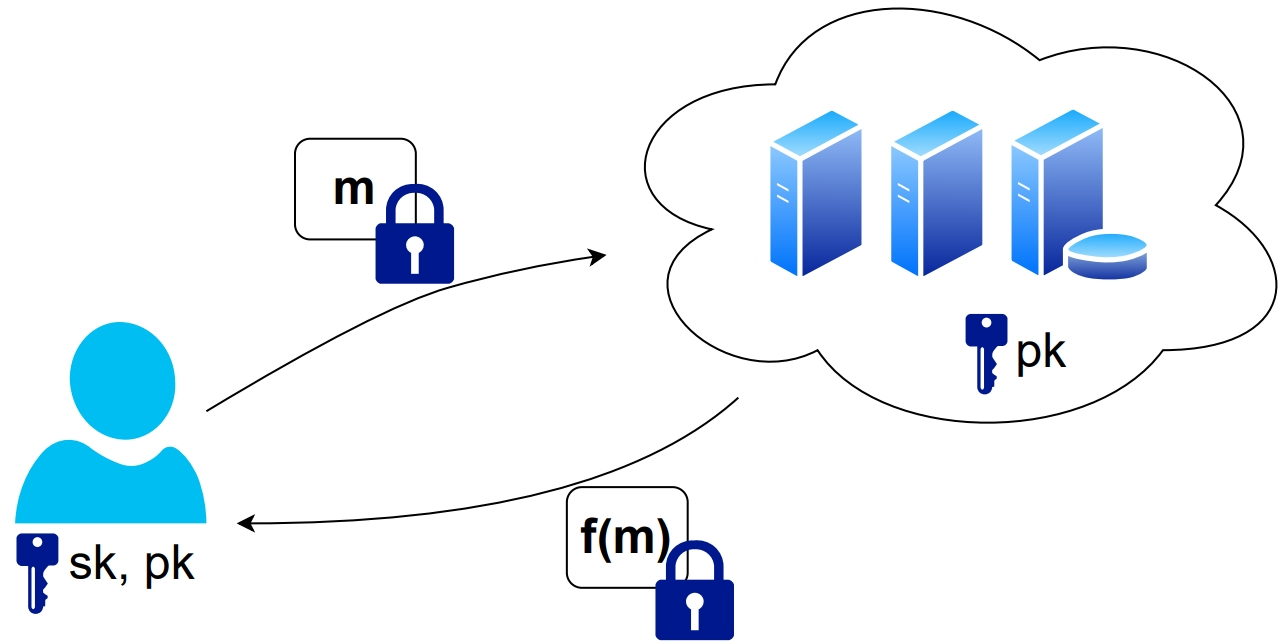
\includegraphics[scale=0.13]{fhe.jpg}
    \caption{Paper:https://ia.cr/2022/657}
    \end{figure}}
    \only<5,6>{
    \begin{figure}[h!]
        \centering
            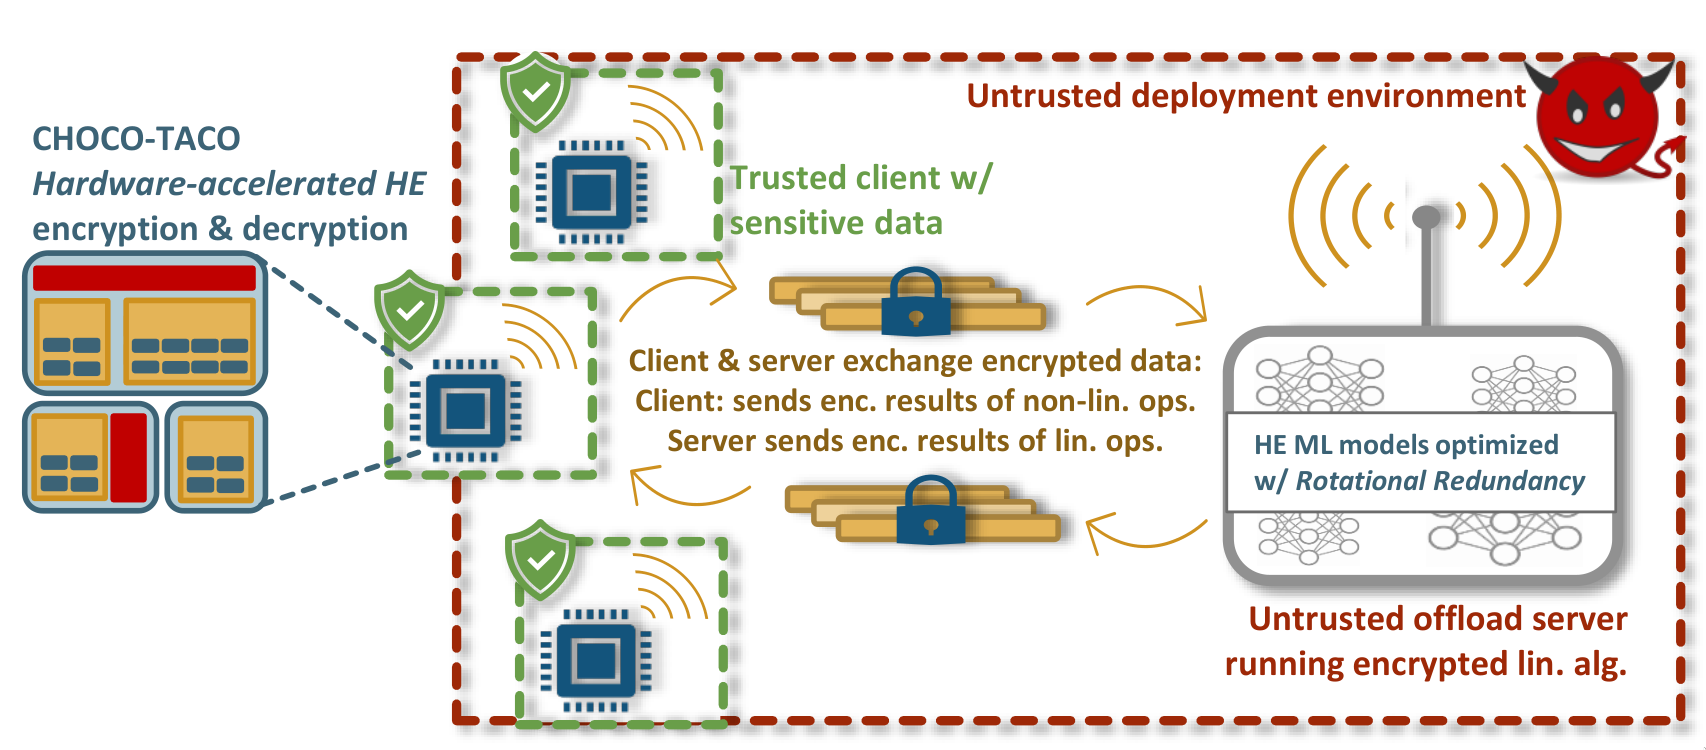
\includegraphics[width=1.\textwidth]{model.png}
    \end{figure}

    }
    \column{0.4\textwidth}
    \begin{itemize}
        \item Client encrypted data (SK).
        \item Send data and PK to server.
        \item Server operates with out decrypt it.
        \item Server send back the result.
        \item Client decrypts the result with SK.
    \end{itemize}
\end{columns}
\pause
\pause
    \vspace{-0.2cm}
    \textbf{Present}: Orders of magnitude \textbf{slower} for real use.
\end{frame}



% ACA PONER COMO ES CLIENT-AIDED?

%%%%%%%%%%%%%%%%%%%%%%%%%%%%%%%%%%%%%%%%%%%%%%%%%%%%%%%%%%%%%%%%%%%%%%%%%%%%%%%%%%%%%%%%%%%%%%%%%%%%


\begin{frame}
    \frametitle{FHE}
    HE supports only addition, multiplication and rotation $\rightarrow$ only \textbf{linear} operations.
\pause
    \vspace{0.3cm}
  \begin{columns}
    \column{0.5\textwidth}
      In general, HE schemes use \texttt{Ring Learning With Errors} (RLWE) that
      \textbf{adds some noise} (error) to the encryption.

\pause
\vspace{0.3cm}
      This \textbf{noise grows} in each operation (particularly with \textbf{multiplications}).

\vspace{0.3cm}
      If the noise is too big will be \textbf{undecryptable}.
\pause
    \column{0.5\textwidth}
        \begin{figure}[h!]
            \centering
            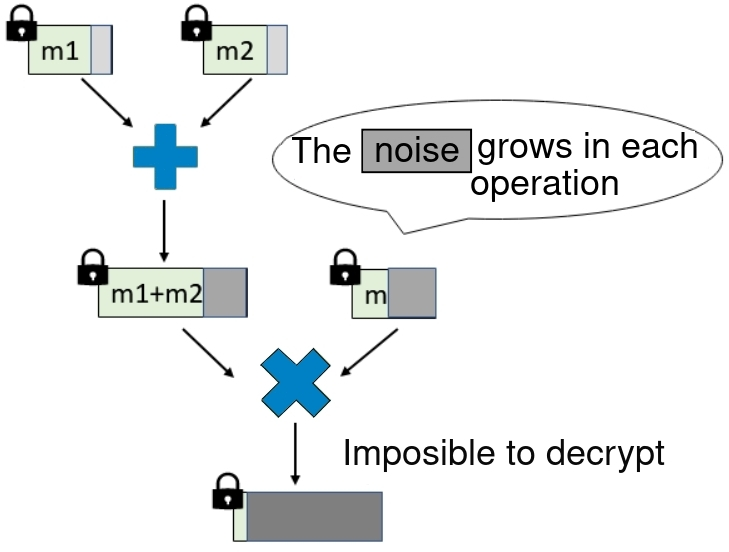
\includegraphics[scale=0.2]{multNoise.jpg}
        \end{figure}



\end{columns}

\pause
    Fully Homomorphic Encryption (FHE): \textbf{Unlimited} number of operations. In this type of schemes
    it use \texttt{Bootstrapping} that are techniques that refresh this error.

\pause
    Even slower!!!
\end{frame}

%%%%%%%%%%%%%%%%%%%%%%%%%%%%%%%%%%%%%%%%%%%%%%%%%%%%%%%%%%%%%%%%%%%%%%%%%%%%%%%%%%%%%%%%%%%%%%%%%%%%


\begin{frame}
    \frametitle{Schemes}
    % ver de agregar algo para batching.

    Many schemes. \textbf{Warning}: Many acronyms!!!

    Popular schemes by types:
    \begin{itemize}\vspace{-0.2cm}
        \item Operations on integers: \textbf{BFV} and BGV.\vspace{-0.2cm}
\pause
        \item Operations on real numbers: CKKS.\vspace{-0.2cm}
        \item Operations on Boolean gates: FHEW and THFHE.
    \end{itemize}

\pause
    \textbf{''Upgrades''}:
\begin{itemize}\vspace{-0.2cm}
    \item Residue Number System (\textbf{RNS}) (stay with 64bits arithmetic's).
        Representation of an input as $k$ \textbf{smaller}  residues of relative primes.
        The Chinese Remainder Theorem (\textbf{CRT}) allows pair-wise operations.
 \vspace{-0.2cm}
\pause
   \item SIMD arithmetic (batching).
\end{itemize}


\end{frame}

%%%%%%%%%%%%%%%%%%%%%%%%%%%%%%%%%%%%%%%%%%%%%%%%%%%%%%%%%%%%%%%%%%%%%%%%%%%%%%%%%%%%%%%%%%%%%%%%%%%%


\begin{frame}
    \frametitle{BFV}
    Works in a \textbf{Polynomial Ring} domain.

 \vspace{-0.25cm}
\textbf{Ring}: a set with addition, subtraction and multiplication. (and other property's, commutative, associative, etc).

\pause
 \vspace{-0.25cm}
    This operations of elements in a ring return elements in the ring $\rightarrow$  \textbf{modular arithmetics}.

 \vspace{-0.25cm}
\textbf{Parameters}: are application-specific and desired security.

\pause
 \vspace{-0.3cm}
\begin{itemize}\itemsep-0.9em
    \item $\lambda$ security level. $\sim$ $2^\lambda$ operation to decrypt with prob 1. (128, 256.)
    \item $N$: the degree of the Polynomials ($N$-1).
        \SubItem{$N$ = 8192, 16384, 32768: $\uparrow$ $N$ $\approx$ $\uparrow$ noise budget, $\uparrow$ ciphertex and comp.}
\pause
    \item $q$ and $t$: the mod of the coefficients.
        \SubItem{$q$ = $2^{218}$,   $2^{438}$,  $2^{881}$: $\uparrow$ $q$ $\approx$ $\uparrow$ noise budget, $\uparrow$ ciphertex, computation.}
        \SubItem{$t$  << $q$: $\downarrow$ $t$ $\approx$ $\uparrow$ noise budget, $\downarrow$ precision.}
\pause
    \item $k$: size of the set of the RNS technique.
        \SubItem{$k\in [3,5], 9, 16$: stay in 64bits arithmetic's, $\uparrow$ parameters, $\uparrow$ $k$.}
\end{itemize}
% q en general es exponencial con la profunidad L.
\pause
\end{frame}


%%%%%%%%%%%%%%%%%%%%%%%%%%%%%%%%%%%%%%%%%%%%%%%%%%%%%%%%%%%%%%%%%%%%%%%%%%%%%%%%%%%%%%%%%%%%%%%%%%%%

% quizas menos.
\begin{frame}
\frametitle{BFV Primitives}

\begin{itemize}\itemsep-0.9em
    \item ParamGen($\lambda$)$\rightarrow$ Default Params.
    \item KeyGen(Params) $\rightarrow$ SK, PK, EvalK (each is a tuple of two polynomials)
        \SubItem{ Sample 3 polynomials, two polynomial multiplication, two additions and two modulus.}
\pause
    \item Encrypt(PK, m) $\rightarrow$ c (tuple of two polynomials)
        \SubItem{ Sample 3 polynomials, two polynomial multiplication, one scalar multiplication, three additions and two modulus.}
    \item Decrypt(SK, c) $\rightarrow$ m
        \SubItem{ similar to Encryption.}
\pause
    \item EvalAdd(c$_1$, c$_2$) $\rightarrow$ c$_3$ (tuple of two polynomials)
    \item EvalMult(c$_1$, c$_2$) $\rightarrow$ c$_{mul}$ (tuple of three polynomials)
\pause
    \item Relinerize(c$_{mul}$, EvalK) $\rightarrow$ c$_{mul}$' (tuple of two polynomials)
        \SubItem{ Six polynomial multiplications, three additions and five modulus.}
\end{itemize}

\end{frame}


%%%%%%%%%%%%%%%%%%%%%%%%%%%%%%%%%%%%%%%%%%%%%%%%%%%%%%%%%%%%%%%%%%%%%%%%%%%%%%%%%%%%%%%%%%%%%%%%%%%%


\begin{frame}
    \frametitle{Bootstrapping tradeoff}

    Approach 1: \textbf{No Bootstrapping}

    Know how many operations are needed (depth level)

    Bigger scheme parameters $\approx$ bigger noise budget $\approx$ slower computation.

\pause
    Approach 2: \textbf{Bootstrapping}

    Use Bootstrapping us needed.

\pause
    Approach 3: \textbf{Client-aided}

    Use the client to decrypt and encrypt again (refresh the noise).
\end{frame}




%%%%%%%%%%%%%%%%%%%%%%%%%%%%%%%%%%%%%%%%%%%%%%%%%%%%%%%%%%%%%%%%%%%%%%%%%%%%%%%%%%%%%%%%%%%%%%%%%%%%

\begin{frame}
\frametitle{Recap}

    \textbf{Remember!} All things are high degree polynomials with huge coefficient.


Each Homomorphic operation is $10^3 \sim 10^6$ times slower than unencrypted.
\pause

Large footprint in memory.
An encrypted date can occupy $10^5$ more space.

\pause

        \begin{figure}[h!]
            \centering
            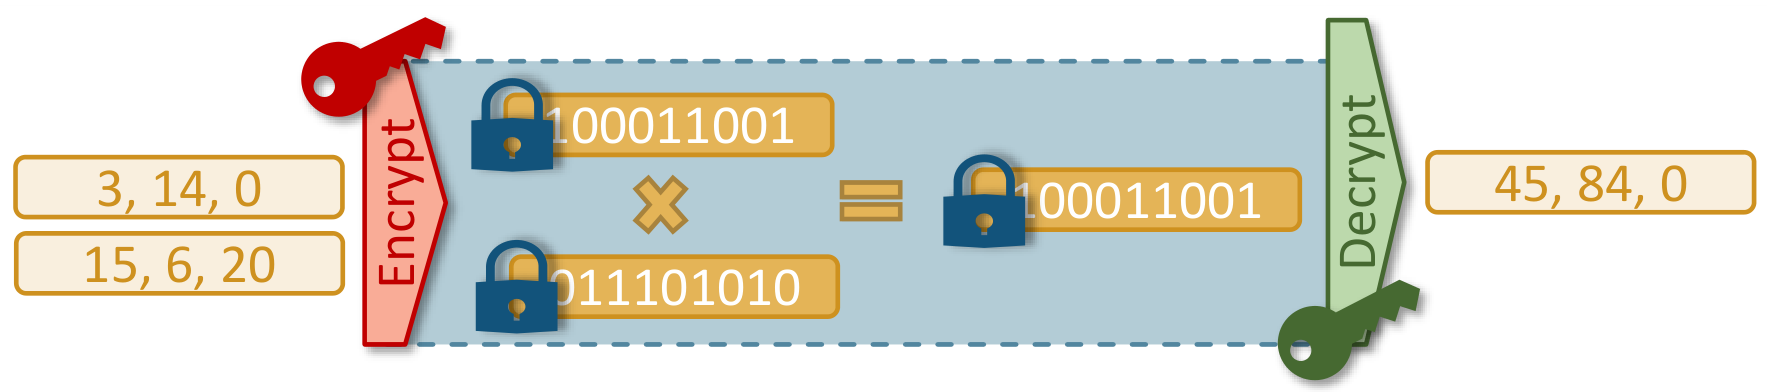
\includegraphics[scale=0.8]{workflow.png}
        \end{figure}
    \centering
        SIMD example


\end{frame}
%%%%%%%%%%%%%%%%%%%%%%%%%%%%%%%%%%%%%%%%%%%%%%%%%%%%%%%%%%%%%%%%%%%%%%%%%%%%%%%%%%%%%%%%%%%%%%%%%%%%


\begin{frame}
\frametitle{Research}

    Usual way of increase performance:  accelerating the server part.
\pause
\begin{itemize}\itemsep-0.7em
   \item New methods of Bootstrapping.
   \item Algorithms implementations, like packed ones (concatenate multiple plaintexts).
       \pause
   \item Accelerating the polynomial multiplication:
       For these they use Number Theoretic Transform (NTT), a Discrete Fourier Transform (DFT) over a ring.
   \item Hardware Acceleration (GPUs, FPGA, specific designs).
\end{itemize}
\pause

    \textbf{Linearity problem}: Approximate with polynomial expansions $\rightarrow$ fast noise growth.
\end{frame}
%%%%%%%%%%%%%%%%%%%%%%%%%%%%%%%%%%%%%%%%%%%%%%%%%%%%%%%%%%%%%%%%%%%%%%%%%%%%%%%%%%%%%%%%%%%%%%%%%%%%


\begin{frame}
\frametitle{New approach}
    \vspace{-0.2cm}
CHOCO: \textbf{C}lient-aided \textbf{H}E for \textbf{O}paque \textbf{C}ompute \textbf{O}ffloading.

    \vspace{-0.2cm}
    Is a \textbf{client-aided} HE: (also use state of art server optimizations)
\pause
    \vspace{-0.4cm}
\begin{itemize}\itemsep-0.7em
    \item Refresh noise when is needed.
    \item Compute non-linear operations (e.g. activation functions in NN).
\end{itemize}

\pause
% para que y cuando se utiliza el rotacional redundancy
    Minimice the client costs: specially encryption and decryption.
    \vspace{-0.2cm}
\begin{itemize}\itemsep-0.7em
        \item Reduces ciphertext size $\rightarrow$ reduces computation and communication costs.
    \item New algorithm: rotational redundancy $\rightarrow$ reduces computation costs.
\pause
    \item Reduction of parameters values $\rightarrow$ reduces computation and communication costs.
    \item Hardware acceleration for client: CHOCO-TACO.
\end{itemize}
% rotational es mas para DNN y demas? o funca para otras cosaS?
%ACLARAR que es mas apra IoT.
\pause
    Testing case: \textbf{DNN} (also shows for: pageRank, K-mean, KNN).

    CHOCO supports unmodified networks with arbitrary activation functions.

\end{frame}


%%%%%%%%%%%%%%%%%%%%%%%%%%%%%%%%%%%%%%%%%%%%%%%%%%%%%%%%%%%%%%%%%%%%%%%%%%%%%%%%%%%%%%%%%%%%%%%%%%%%

\section{Research}

%\begin{frame}
%\frametitle{Motivation}
%
%
%UNIR ESTAS DOS DIAPOS
%
%The most clear example: DNN inference.
%% they use a lot, and things like rotational seems to be boosted.
%
%    \textbf{Before}: No client intermediate communication $\rightarrow$ adapt networks architecture and approximations of non-linear operations.
%
%    \textbf{Problems}: Fast noise accumulation, large HE parameters, big ciphertext (more costly to process and communication)
%
%CHOCO:
%\begin{itemize}
%    \vspace{-0.2cm}  \item Client-aided $\rightarrow$ offload linear convolution and fully-connected layers to HE server.
%    \vspace{-0.2cm}\item Send intermediate results to the client to perform non-linear operations and refresh noise.
%    \vspace{-0.2cm}\item Supports unmodified networks with arbitrary activation functions.
%\end{itemize}
%
%Larger client cost!
%CHOCO minimize this cost (with also CHOCO-TACO).
%
%\end{frame}


%%%%%%%%%%%%%%%%%%%%%%%%%%%%%%%%%%%%%%%%%%%%%%%%%%%%%%%%%%%%%%%%%%%%%%%%%%%%%%%%%%%%%%%%%%%%%%%%%%%%

% Quizas esta vuela por que despues hay otra parecida usando CHOCO
\begin{frame}
\frametitle{Benchmark}
% NO USAN CHOCO aca
% ARM 1.2Ghz, 100mw, 28nm
\begin{columns}
    \column{0.5\textwidth}
    \textbf{CPU Client}: ARM cortex-A7
    \vspace{0.1cm}

    \textbf{Workload}: single image DNNs inference, 4 different models.
\pause
    \column{0.5\textwidth}
    \textbf{Profile}: 60\% is on polynomial multiplication and NTT of SEAL encryption and decryption.
\end{columns}

\pause
% HEAX is a NTT accelerator.
% State of art encryption and decryption accelerator in FPGA.
\begin{columns}
    \column{0.8\textwidth}
\begin{figure}
    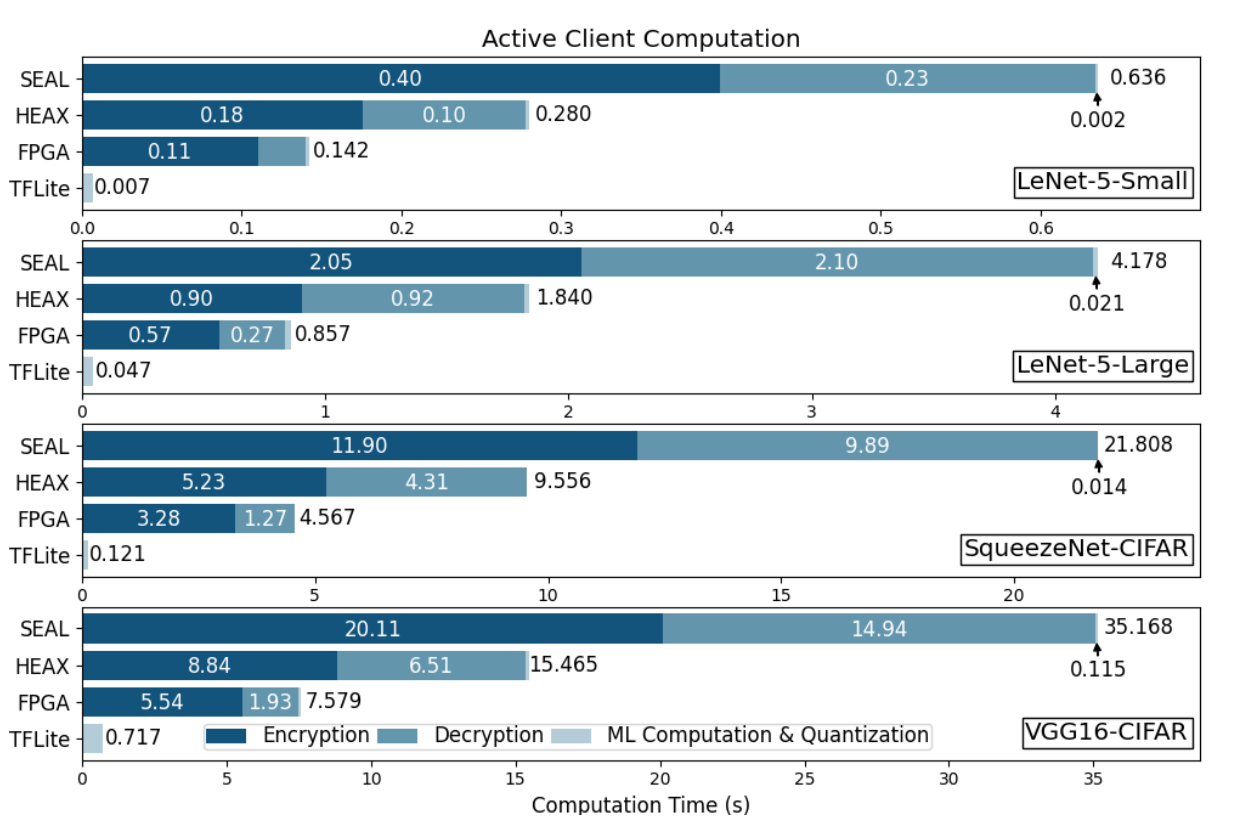
\includegraphics[width=0.85\textwidth]{motivation.png}
\end{figure}
    \vspace{-0.5cm}
    \column{0.2\textwidth}
\pause
99\% of client compute HE operations.
    \vspace{0.3cm}

Up to 180x overhead to offload compute.
\end{columns}
\centering

% Lo que muestra aca es la diferencia entre lo que tarda la Encrpytion y decryption en el cliente
% vs lo otro

\end{frame}


%%%%%%%%%%%%%%%%%%%%%%%%%%%%%%%%%%%%%%%%%%%%%%%%%%%%%%%%%%%%%%%%%%%%%%%%%%%%%%%%%%%%%%%%%%%%%%%%%%%%


\begin{frame}
\frametitle{Algorithm optimizations}
% como hicieron para usar un valor menos de k?
    \textbf{Reduce parameters} $\rightarrow$Efficient HE Parameters $\rightarrow$ aggressive 4-bits input quantification.
    % primero discretizo los inputs y depsues lo paso a plaintext y demas.
    \vspace{-0.2cm}

    \pause
Packed HE algorithms $\rightarrow$  aligned vectors to operate in the desire way.
    \vspace{-0.2cm}

Rearrange encrypted vectors $\rightarrow$ rotations and multiplications  $\rightarrow$ Noise grows a lot!

    \pause
    \vspace{-0.2cm}
%Convolutions use a lot of rotations. Explica como lo usaron...
    New algorithm! \textbf{Rotational Redundancy} $\rightarrow$ lower arithmetic depth $\rightarrow$ less noise.

    \vspace{-0.2cm}
    50\% smaller ciphertext $\rightarrow$ $k$-1 $\rightarrow$ 1.7x speed, remains 62x overhead vs TFLite.
    \vspace{-0.2cm}
    \pause
% por ser ciphertext hay que rotar todo y no solo la ventanita que queremos.
\begin{figure}
    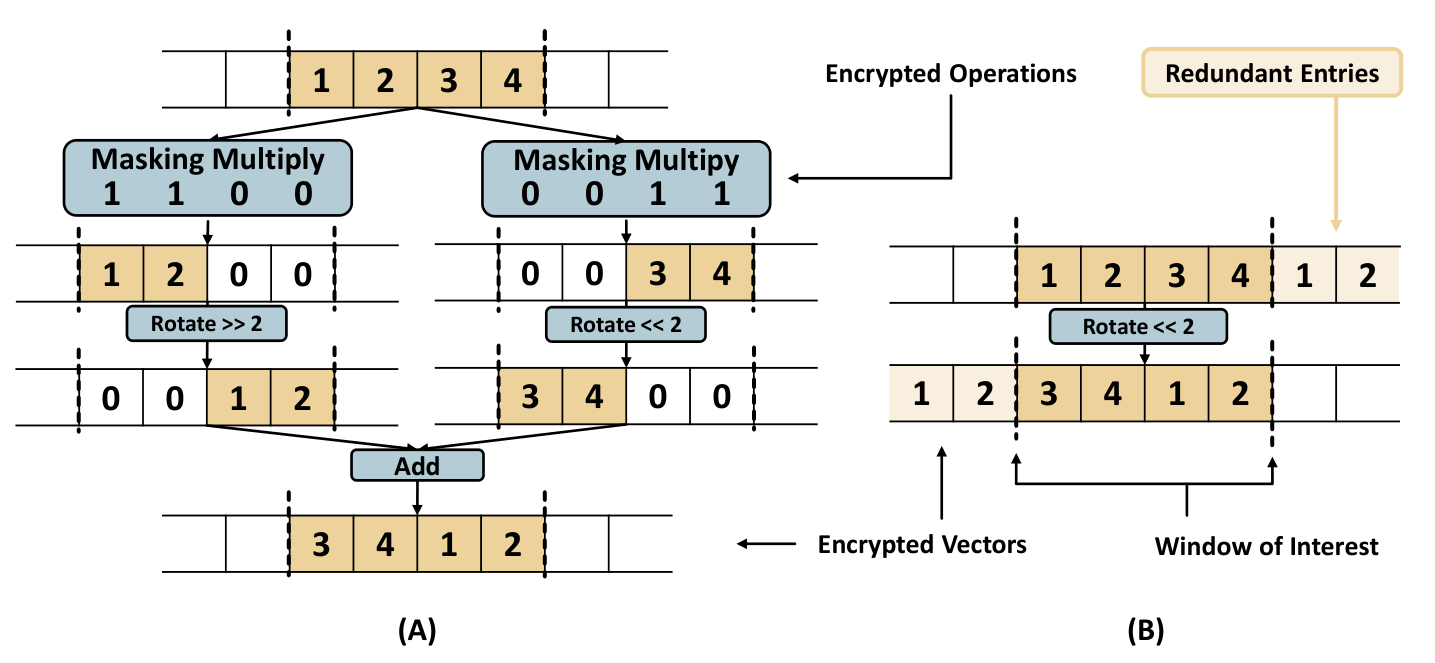
\includegraphics[width=0.85\textwidth]{rotation.png}
\end{figure}
    % RGB is 3 channel or each convolution layer)
\end{frame}

%%%%%%%%%%%%%%%%%%%%%%%%%%%%%%%%%%%%%%%%%%%%%%%%%%%%%%%%%%%%%%%%%%%%%%%%%%%%%%%%%%%%%%%%%%%%%%%%%%%%


%\begin{frame}
%\frametitle{Rotational Redundancy - CHOCO}
%Exploits the fact that the client  always decrypt, unpack, repack and encrypt.
%
%So client discard redundant data adds new values for the next operation.
%
%Typically the redundancy is a small fraction of the total vector size.
%
%Convolution requieres windowed rotation within each channel.
%
%CHOCO packs each channel of an image with sufficient redundancy to keep
%values aligned through the encrypted convolution.
%
%CHOCO stacks the redundan channel vector into evenly-spaced, power-of-two-sized slots in the final ciphertext vector.
%
%All elements can be properly aligned for convolution.
%
%50\% reduction of ciphertext size compared to SEALS with same N=8192.
%
%One less  RNS entry.


% FPGA implementation
%\end{frame}
%%%%%%%%%%%%%%%%%%%%%%%%%%%%%%%%%%%%%%%%%%%%%%%%%%%%%%%%%%%%%%%%%%%%%%%%%%%%%%%%%%%%%%%%%%%%%%%%%%%%


\begin{frame}
\frametitle{CHOCO-TACO}
CHOCO + FPGA Encrypt and Decrypt = 4.4x, remain 22x.
    \vspace{-0.2cm}

CHOCO-TACO: \textbf{T}hrough \textbf{A}ccelerated \textbf{C}ryptographic \textbf{O}perations
    \vspace{-0.2cm}

\pause
Accelerates all of the componentes sub-operations of HE encryption and decryption.
    \vspace{-0.2cm}

Virtually eliminates these client costs.
    \vspace{-0.2cm}

\pause
CHOCO-TACO is for BFV and CKKS.
    \vspace{-0.2cm}


 Straightforward, parallel, pipelined hardware, minimal data movement.
    \vspace{-0.2cm}

\pause

 Modules: Pseudo-Random Number Generation, Polynomial Multiplication, Polynomial Addition, Modulus Switching and Message Encoding.
    \vspace{-0.2cm}

 Each module: memories and functional blocks.
    \vspace{-0.2cm}

Each block: processing elements for individual coefficients.
 % Modulus Switching

% al multiplicar dos polynomios en el espacio NTT es simplemente elemento a elemento C[i] = A[i]*B[i]. y despues
% transformamos de nuevo con INTT

\end{frame}

%%%%%%%%%%%%%%%%%%%%%%%%%%%%%%%%%%%%%%%%%%%%%%%%%%%%%%%%%%%%%%%%%%%%%%%%%%%%%%%%%%%%%%%%%%%%%%%%%%%%


\begin{frame}
\frametitle{CHOCO-TACO}

\only<1>{
\begin{equation*}
    Enc([P_0,P_1],m) = ([\triangle m + P_0\textcolor{red}{u}+\textcolor{red}{e_1}]_q, [P_1\textcolor{red}{u}+\textcolor{red}{e_2}]_q)
\end{equation*}
    \begin{figure}
        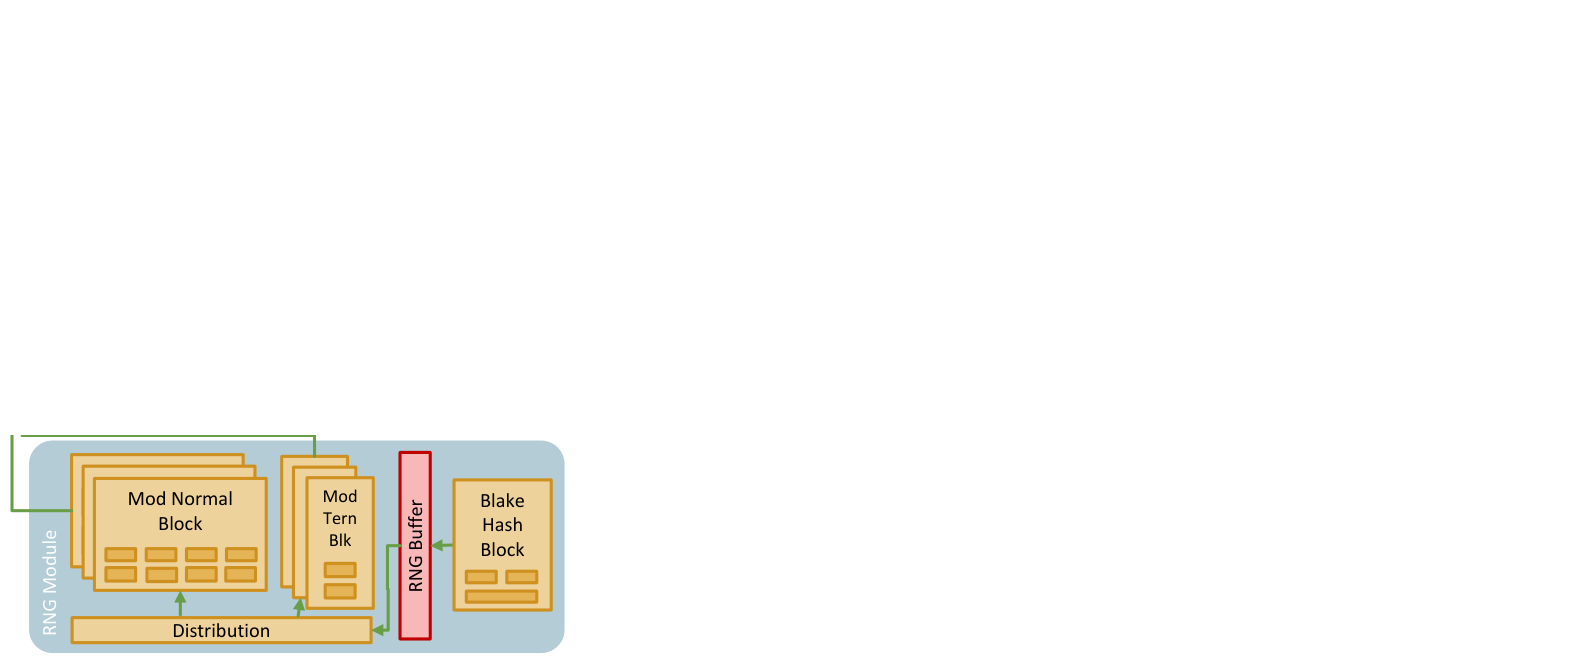
\includegraphics[width=1.0\textwidth]{architecture0.png}
    \end{figure}
}
% random vectors to a NTT transformation.
% initial buffer contains the PK and do multiplication.
% pruductos go to an INTT to then add
    \only<2>{
\begin{equation*}
    Enc([P_0,P_1],m) = ([\triangle m + \textcolor{red}{P_0u}+e_1]_q, [\textcolor{red}{P_1u}+e_2]_q)
\end{equation*}
    \begin{figure}
        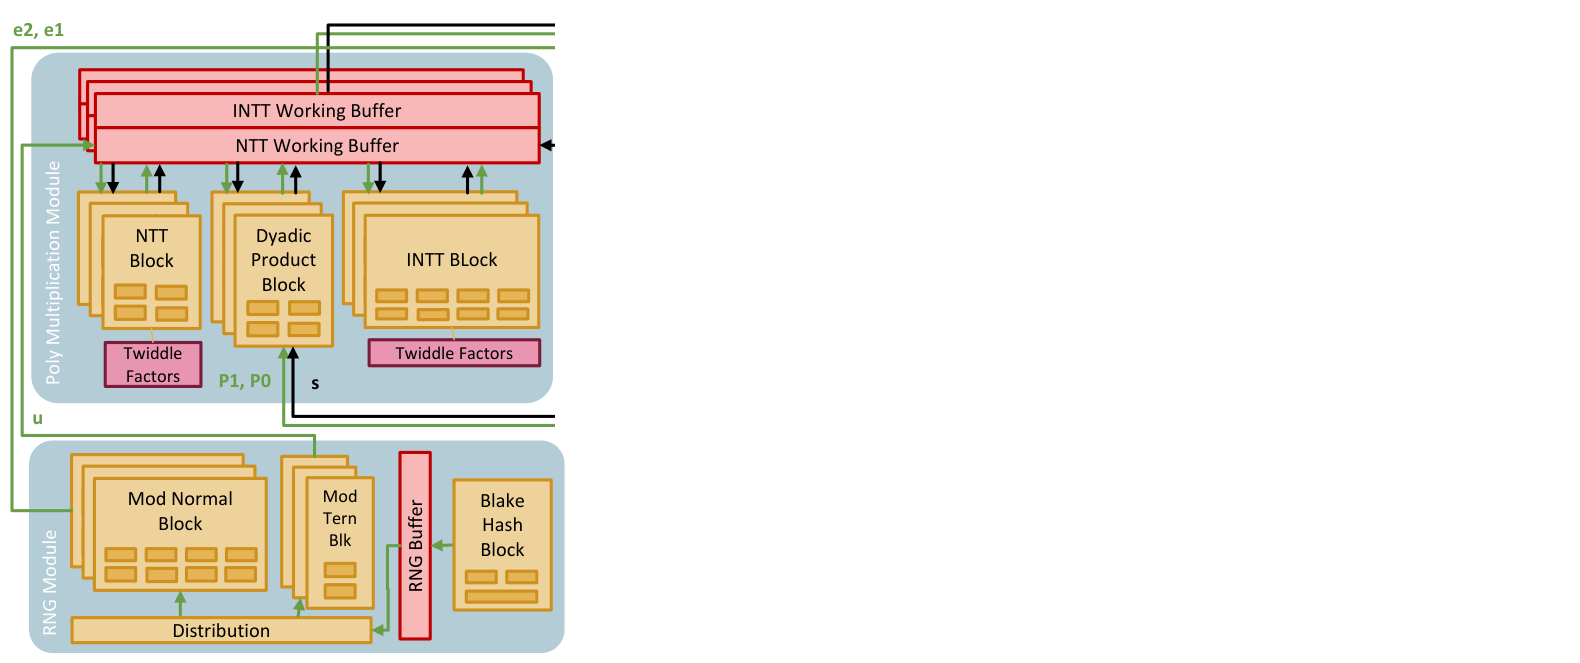
\includegraphics[width=1.0\textwidth]{architecture1.png}
    \end{figure}
}
% c1 is ready.
\only<3>{
\begin{equation*}
    Enc([P_0,P_1],m) = ([\triangle m + \textcolor{red}{P_0u+e_1}]_q, \textcolor{red}{[P_1u+e_2]_q})
\end{equation*}
    \begin{figure}
        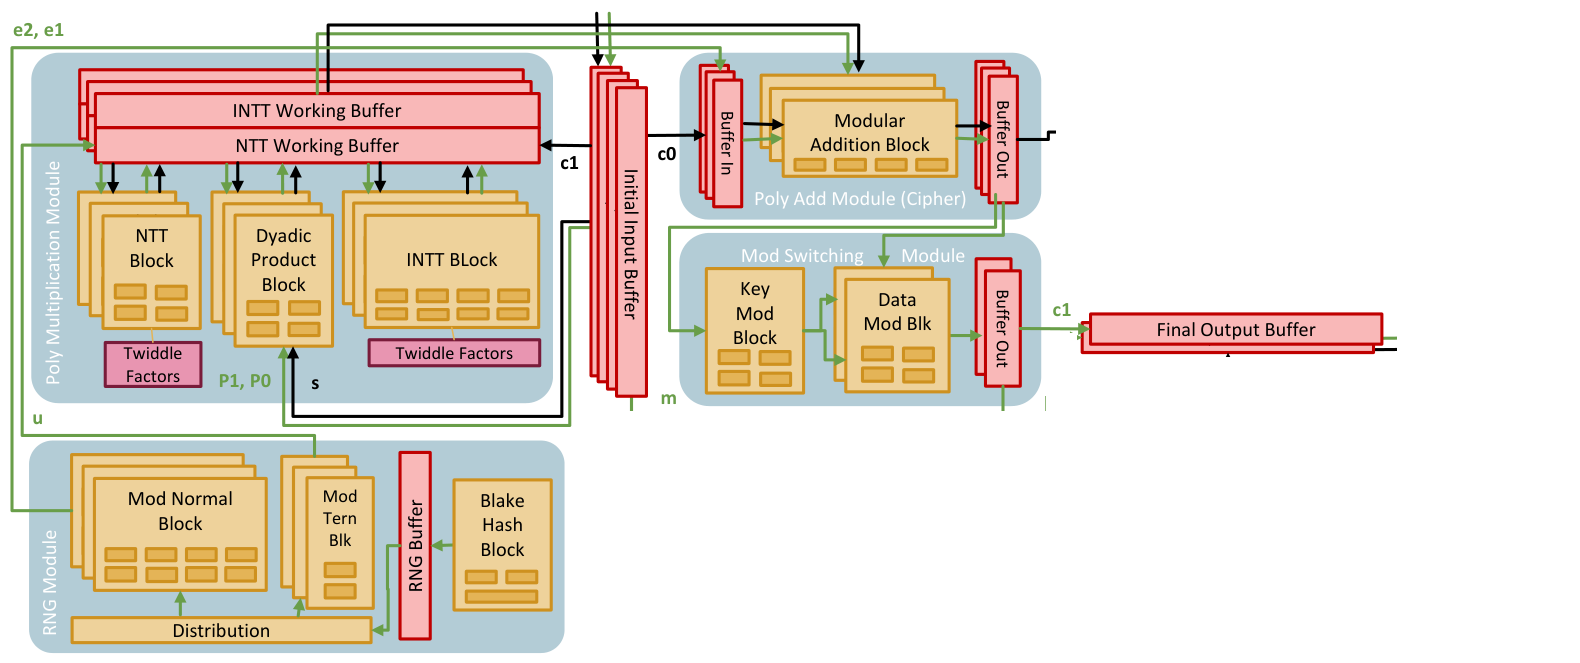
\includegraphics[width=1.0\textwidth]{architecture2.png}
    \end{figure}
}
\only<4>{
    \begin{equation*}
        Enc([P_0,P_1],m) = ([\textcolor{red}{\triangle m} + P_0u+e_1]_q, [P_1u+e_2]_q)
\end{equation*}
    \begin{figure}
        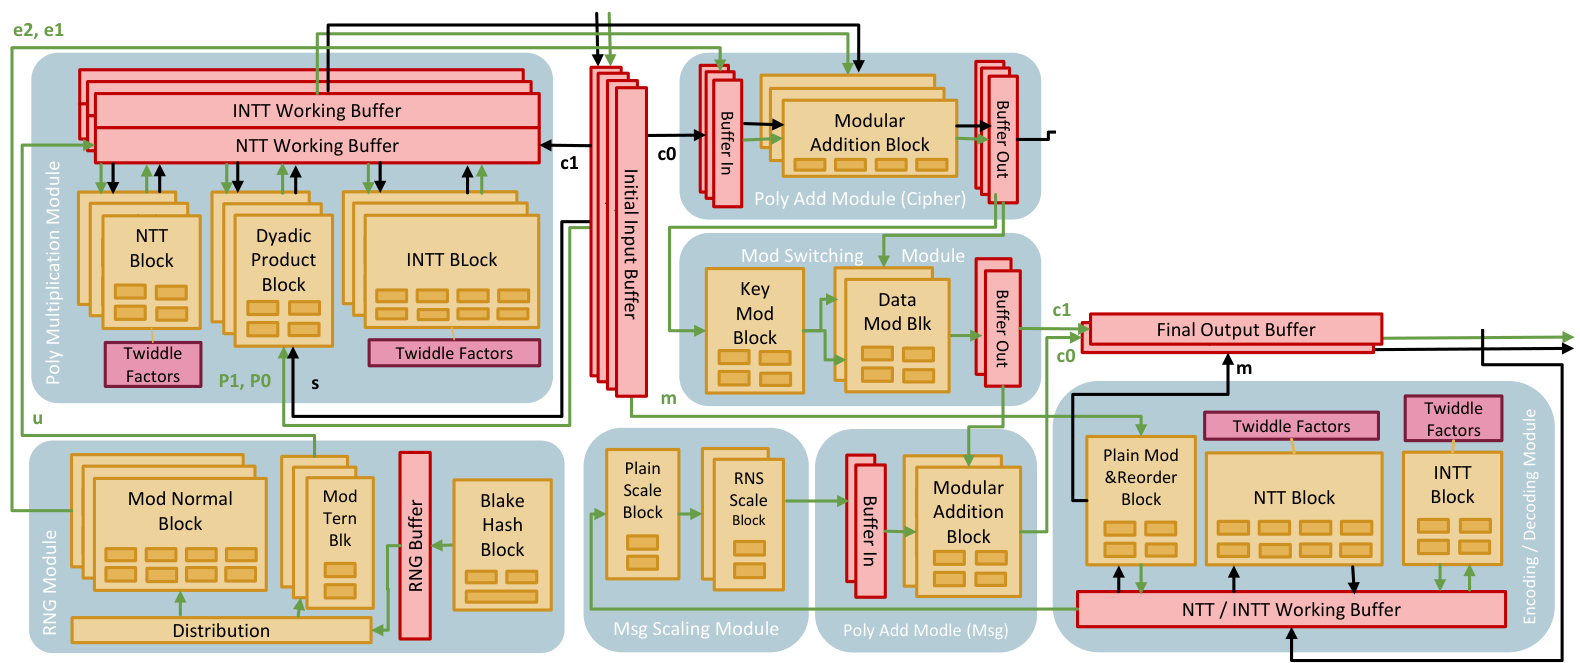
\includegraphics[width=1.0\textwidth]{architecture3.png}
    \end{figure}
}
\only<5>{
\begin{equation*}
    Dec(SK,[c_0,c_1]) = \left[ \left\lfloor \frac{t}{q}[c_0+c_1SK]_q\right\rceil \right]_t
\end{equation*}
    \begin{figure}
        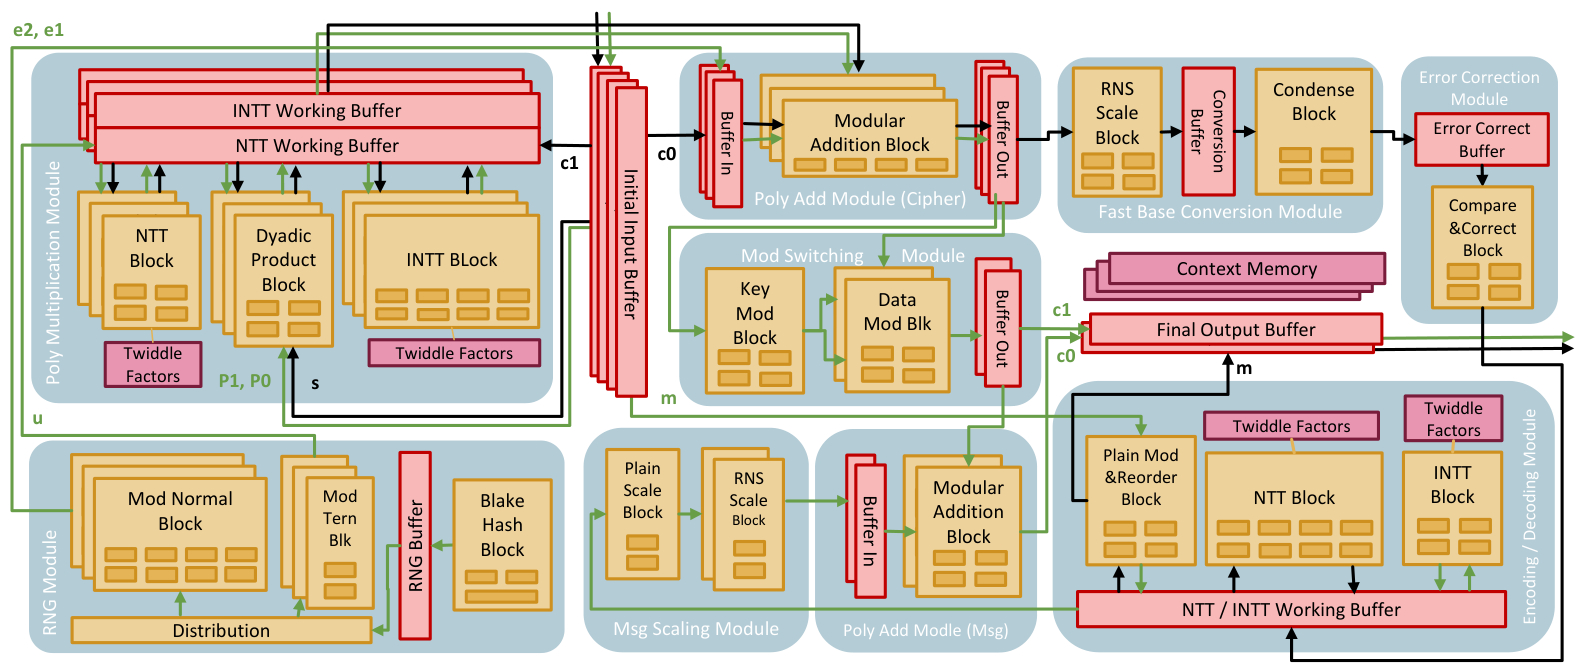
\includegraphics[width=1.0\textwidth]{architecture4.png}
    \end{figure}
}
\only<6>{ Encryption 1094x time and 648x energy (over SW).

    \vspace{-0.2cm}
    Decryption (Less parallelism) only 125x time.
    \begin{figure}
        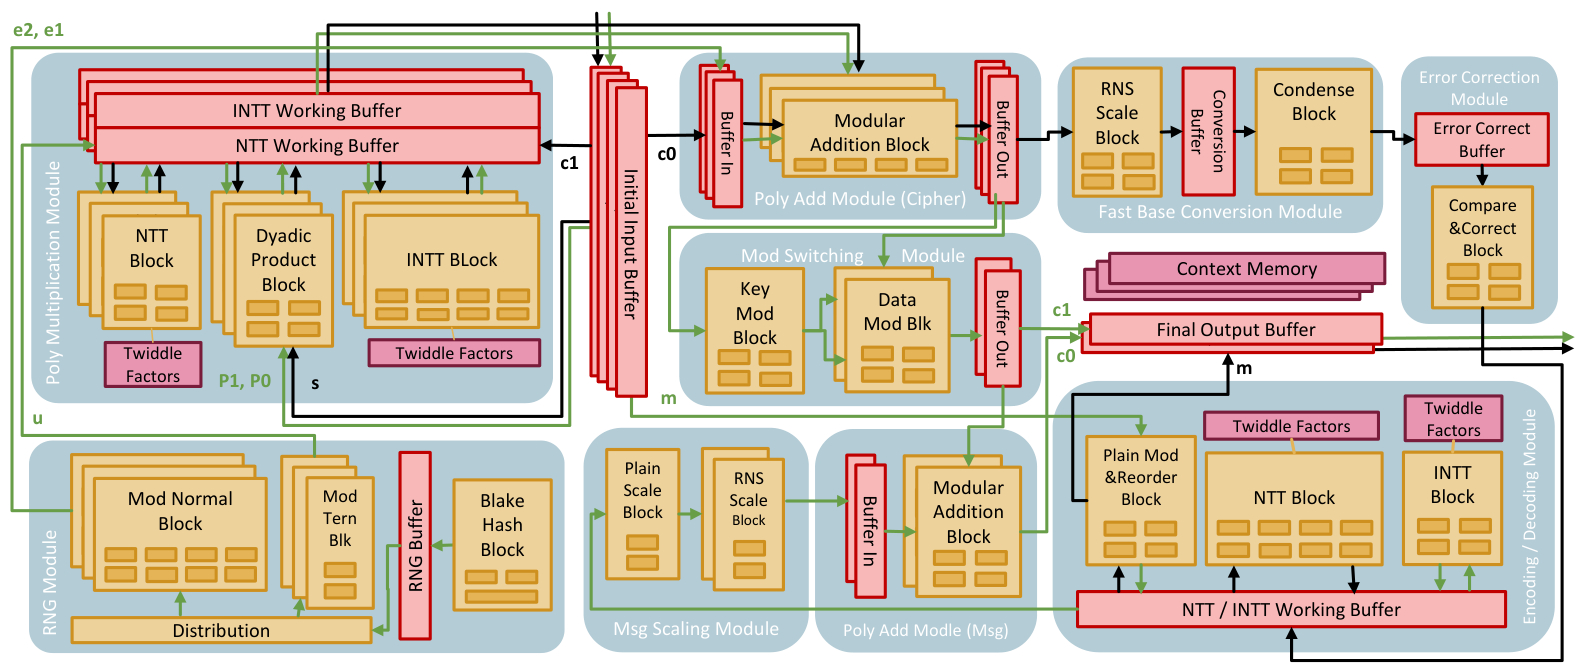
\includegraphics[width=1.0\textwidth]{architecture4.png}
    \end{figure}
}
% Hablar del paralelismo, que hay multiples capas,  SRAM buffers para evitar el movimiento
% iunecesario de data.


\end{frame}


%%%%%%%%%%%%%%%%%%%%%%%%%%%%%%%%%%%%%%%%%%%%%%%%%%%%%%%%%%%%%%%%%%%%%%%%%%%%%%%%%%%%%%%%%%%%%%%%%%%%


\begin{frame}
\frametitle{Design space}
%quizas sacar el grafico que no dice mucho.
Simulation of 31340 different architectural configurations.

Implementation:
\pause
\begin{itemize}
    \item Individual Hardware components in RTL.
    \item Synthesized with Cadence genus in 45nm technology node.
\pause
    \item Model memory with Destiny. SRAM as aggressive wire technology.
    \item Clock: 100MHz for energy optimization.
\end{itemize}


\pause
Select 200mW and smallest design with run time within 1\% of optimal time and energy.

19.3mm$^2$ area and consumes 0.1228mJ to perform single encryption in 0.66ms for N = 8192 and k = 3.
% implement in  RTL individual hatdware components.
% synthesized them with cadence genus in 45nm technology node.
% model memory with destiny, SRAM as aggresive wire techonlogy.
% optmized for read energyy with 8-word,64byte, memory accces.
%clocked 100Mhz for energy optimization.
\end{frame}






%%%%%%%%%%%%%%%%%%%%%%%%%%%%%%%%%%%%%%%%%%%%%%%%%%%%%%%%%%%%%%%%%%%%%%%%%%%%%%%%%%%%%%%%%%%%%%%%%%%%


\begin{frame}
    \frametitle{Client compute Acceleration}
    % SW CHOCO 1.7x over SEAL
    % lower baseline local TFLite compute, UPPER SEAL.
    % TFLite 121x over CHOCO SW show clear bottleneck in encrypt and decrypt.
    % EVEN with HEAX (NTT boost) still 14.5x slower than tflite.
    % WITH TACO that optimil allocation of compute resourcesm, minimal buffering,
    % tightly integrated memories anjd multiple levels opf parrallelism to address the
    % remaining 40% of computation.
    % TACO 2.2x faster thab TFLite.
\begin{columns}
    \column{0.8\textwidth}
    \begin{figure}
        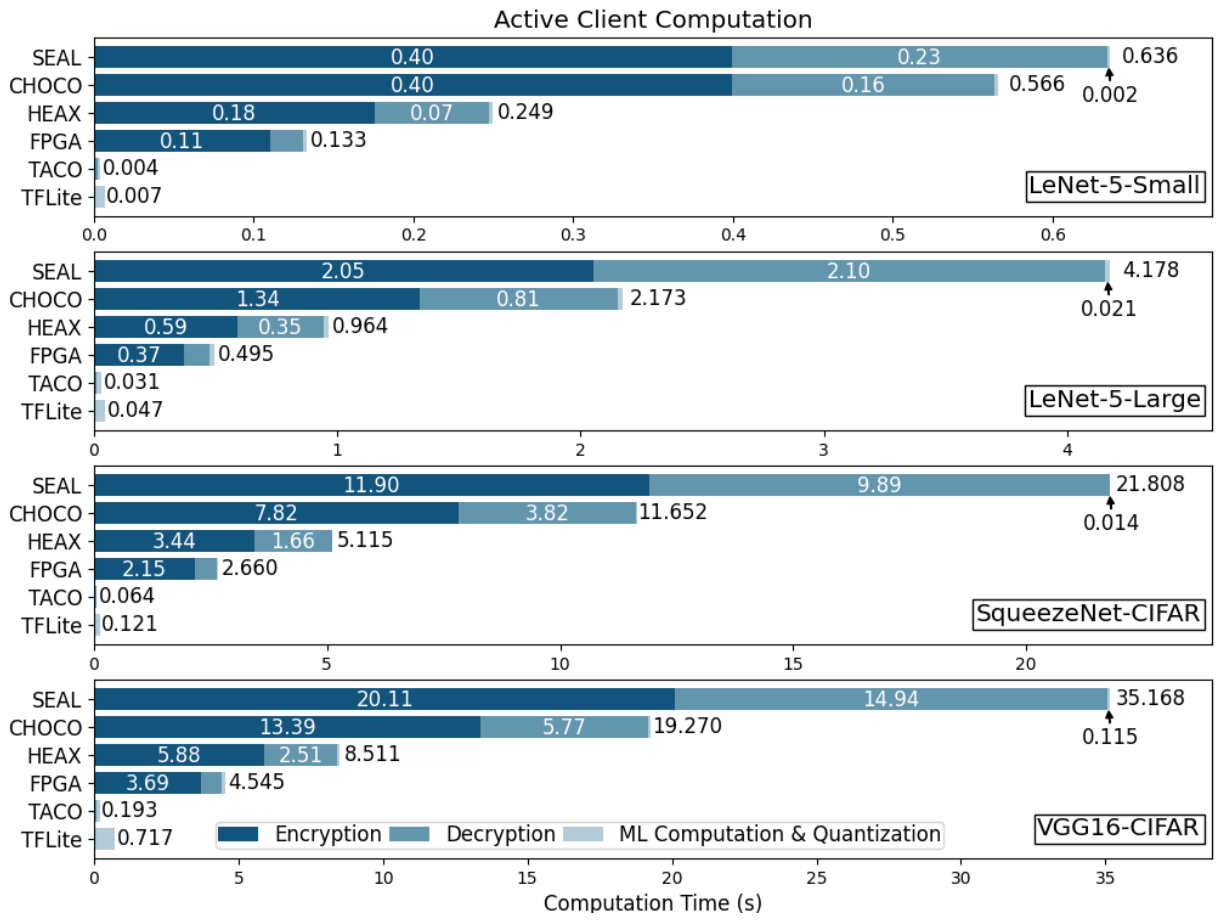
\includegraphics[width=0.95\textwidth]{motivation2.png}
    \end{figure}
\column{0.2\textwidth}
\pause
182x better to CHOCO.
    \vspace{0.3cm}

29x better to CHOCO+FPGA

    \vspace{0.3cm}
2.2x better than local compute.
\end{columns}


\end{frame}
%%%%%%%%%%%%%%%%%%%%%%%%%%%%%%%%%%%%%%%%%%%%%%%%%%%%%%%%%%%%%%%%%%%%%%%%%%%%%%%%%%%%%%%%%%%%%%%%%%%%

\begin{frame}
    \frametitle{Competitive Compute}
    10mW Bluetooth communication at 22Mbps.

    % 24x average time overhead compared to local compute.
    % in small devices battery preservation oftenb outweights the need for fast compute.
    % CHOCO and TFLite is competitive. in VGG 37% savings.
    \begin{figure}
        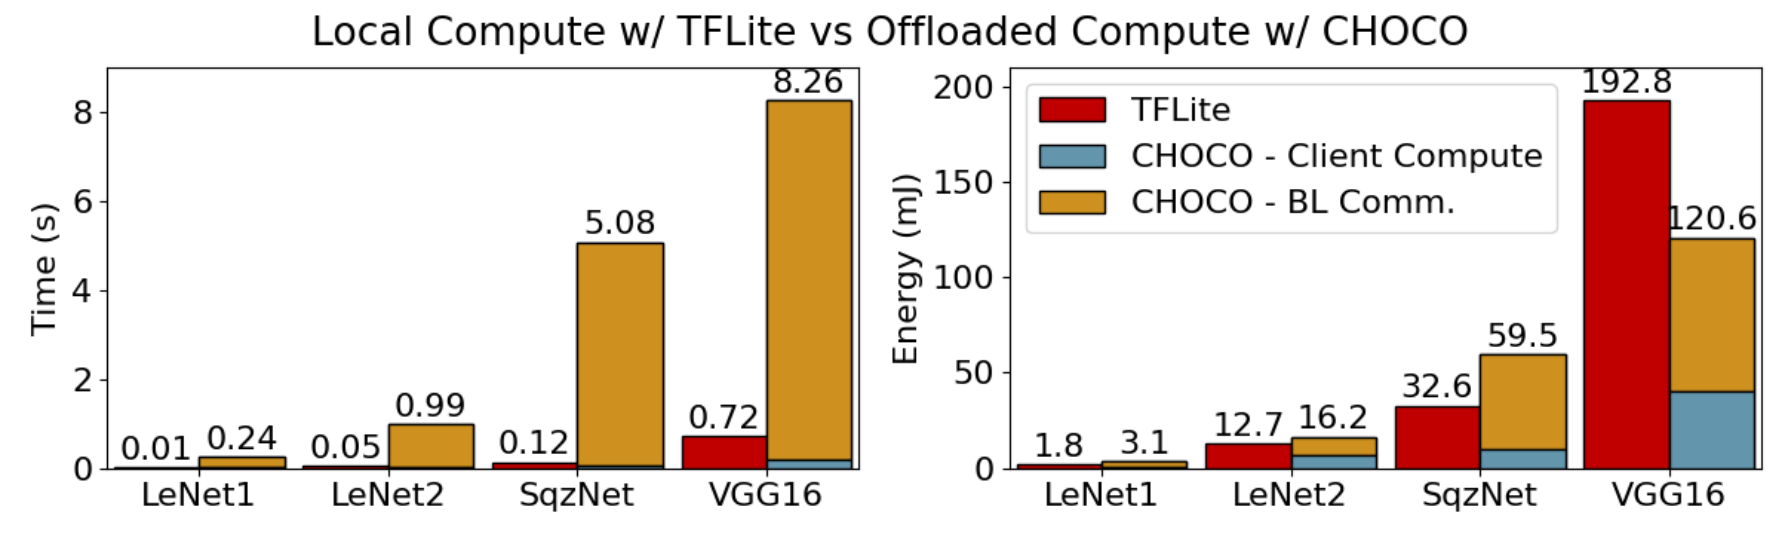
\includegraphics[width=1\textwidth]{energy.png}
    \end{figure}
\pause
37\% decrease energy consumption for VGG16.

    Communications still is a challenge. CHOCO 66\% reduction over SEAL.


\end{frame}

%%%%%%%%%%%%%%%%%%%%%%%%%%%%%%%%%%%%%%%%%%%%%%%%%%%%%%%%%%%%%%%%%%%%%%%%%%%%%%%%%%%%%%%%%%%%%%%%%%%%



\begin{frame}
    \frametitle{Communication reduction}

    \begin{figure}
        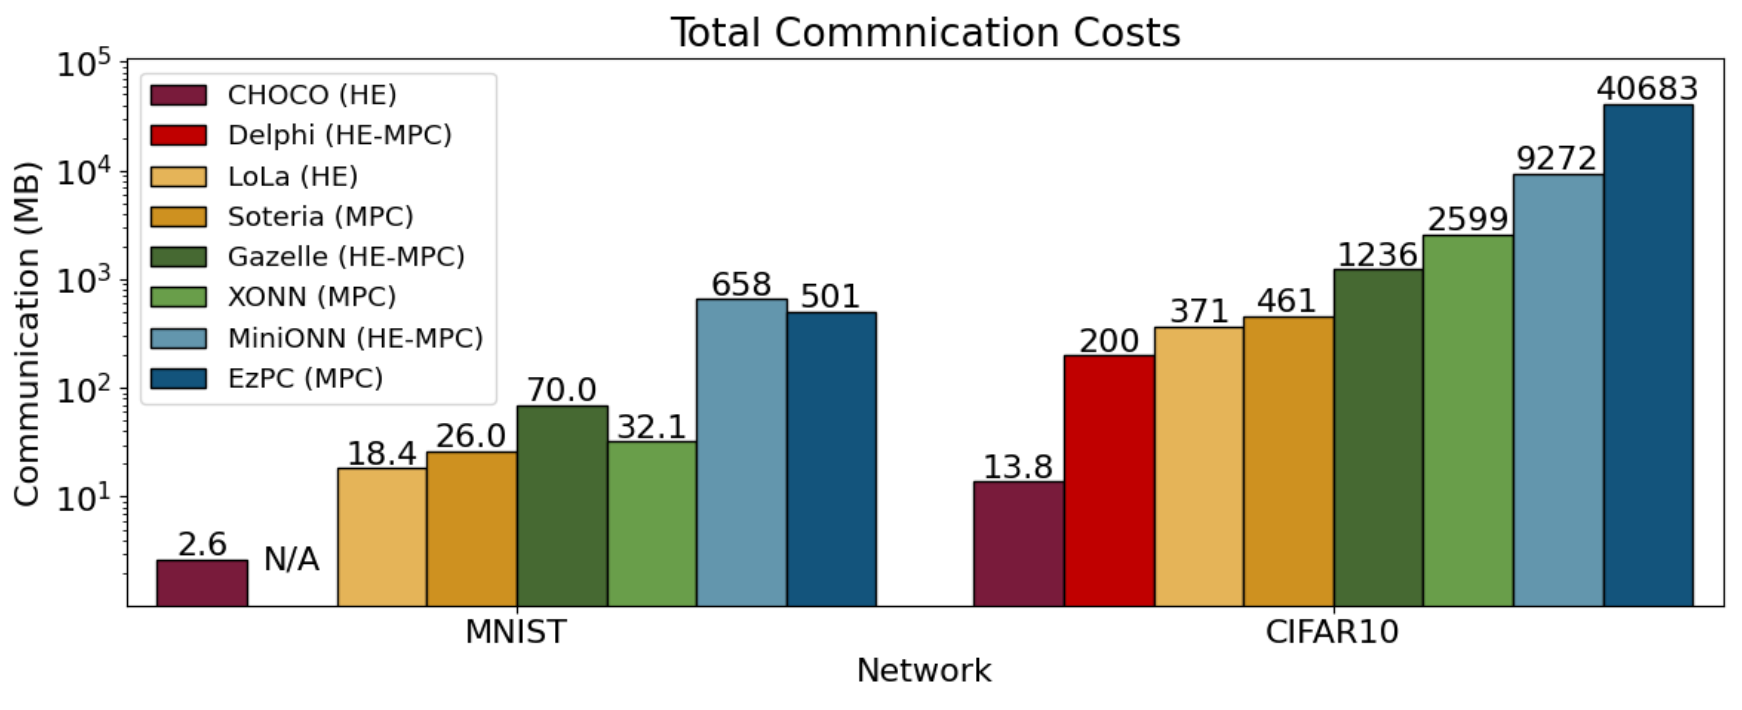
\includegraphics[width=0.95\textwidth]{comunication.png}
    \end{figure}
CHOCO outperforms existing protocols up to three orders of magnitude.

% gazelle es basicamente ujna implementacion de CNN
    90x improvement in communication overhead over Gazelle (CIFAR10).
\pause

    Even better than LoLa (Non-client-aided) by 27x.
    % Lola Non-client
\end{frame}
%%%%%%%%%%%%%%%%%%%%%%%%%%%%%%%%%%%%%%%%%%%%%%%%%%%%%%%%%%%%%%%%%%%%%%%%%%%%%%%%%%%%%%%%%%%%%%%%%%%%
%\begin{frame}
%\frametitle{}
%    \begin{figure}
%    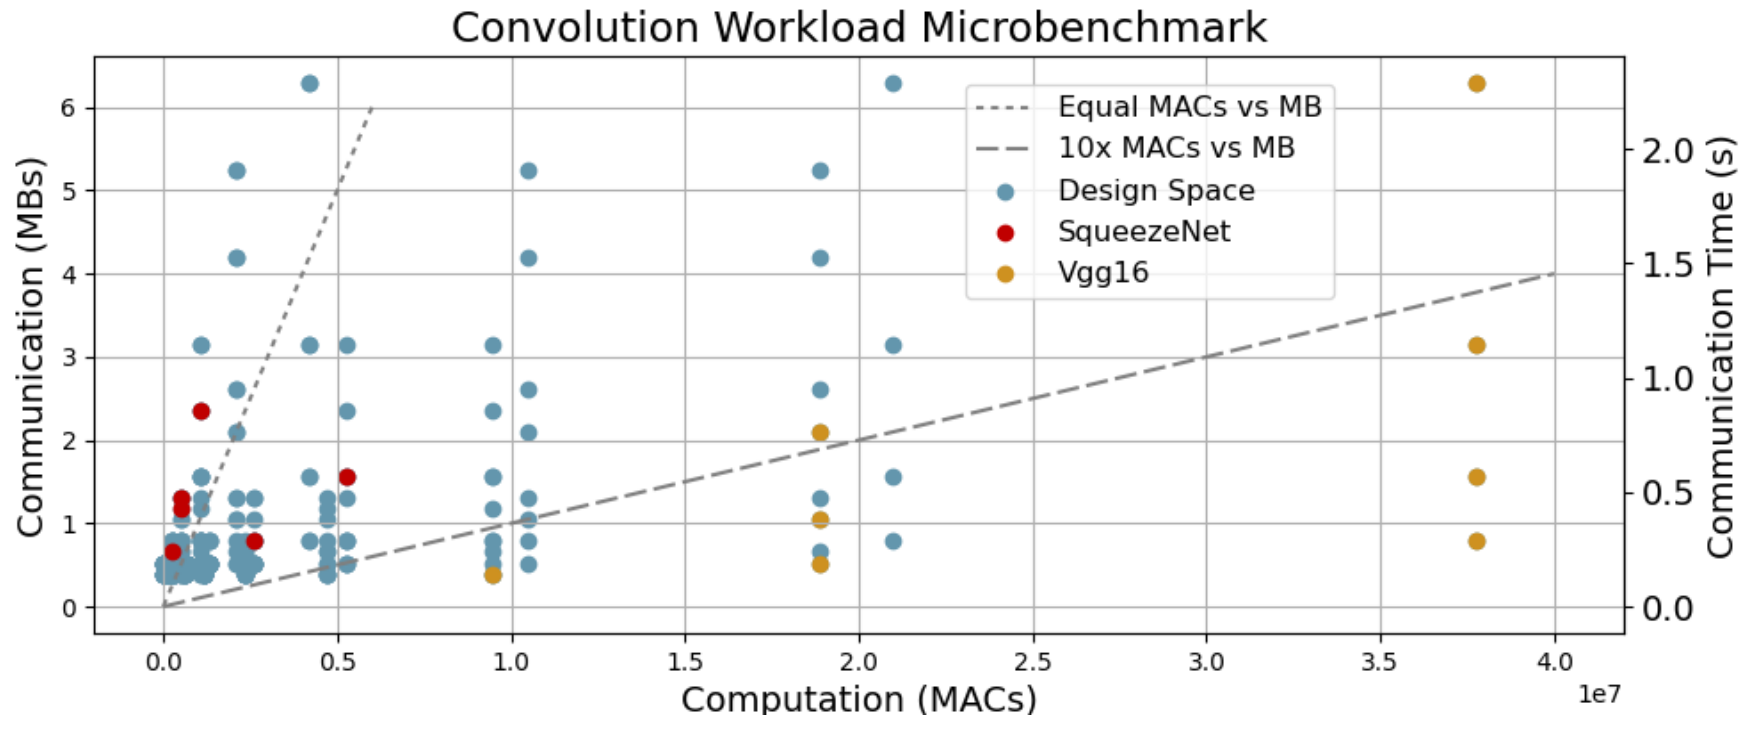
\includegraphics[width=0.95\textwidth]{comunication2.png}
%\end{figure}
%
%
%
%\end{frame}
%%%%%%%%%%%%%%%%%%%%%%%%%%%%%%%%%%%%%%%%%%%%%%%%%%%%%%%%%%%%%%%%%%%%%%%%%%%%%%%%%%%%%%%%%%%%%%%%%%%%

\section{Conclusion}
\begin{frame}
\frametitle{Conclusion}
\begin{itemize}
    \item CHOCO motivates and prioritizes client-aided optimization.
    \item CHOCO algorithm optimizations reduce communication by orders of magnitude over prior work.
\pause
    \item CHOCO-TACO hardware comprehensively accelerates client-side HE.
    \item CHOCO enables participation from resource-constrained devices in client-aided encryption computation.
\pause
    \item CHOCO makes client responsibility competitive with local compute.
    \item Communications still a Bottleneck.
\end{itemize}

\end{frame}
%%%%%%%%%%%%%%%%%%%%%%%%%%%%%%%%%%%%%%%%%%%%%%%%%%%%%%%%%%%%%%%%%%%%%%%%%%%%%%%%%%%%%%%%%%%%%%%%%%%%


\begin{frame}
\frametitle{}
\Huge

\begin{center}
   Questions?
\end{center}
\end{frame}


%%%%%%%%%%%%%%%%%%%%%%%%%%%%%%%%%%%%%%%%%%%%%%%%%%%%%%%%%%%%%%%%%%%%%%%%%%%%%%%%%%%%%%%%%%%%%%%%%%%%

%%%%%%%%%%%%%%%%%%%%%%%%%%%%%%%%%%%%%%%%%%%%%%%%%%%%%%%%%%%%%%%%%%%%%%%%%%%%%%%%%%%%%%%%%%%%%%%%%%%%

% Quizas al pedo.
\begin{frame}[noframenumbering]
\frametitle{Math notation}
BFV, BGV and CKKS works with ciphertex  $\in \mathcal{R}_q =\mathbb{Z}_q[X]/(X^N+0)$

$\mathbb{Z}[X]$ = Set of Polynomials with integer coefficients.

$\mathbb{Z}_q[X]$ = Set of Polynomials with integer coefficients mod q.

$\mathbb{Z}_q[X]/(X^N+0)$ = The Polynomials degree N-1.


\end{frame}
%%%%%%%%%%%%%%%%%%%%%%%%%%%%%%%%%%%%%%%%%%%%%%%%%%%%%%%%%%%%%%%%%%%%%%%%%%%%%%%%%%%%%%%%%%%%%%%%%%%%

%quizas tampoco
\begin{frame}[noframenumbering]
\frametitle{Workflow}

    Encryption has two phases:
\begin{itemize}
    \item From an integer m to plaintext
    \item From plain text to ciphertext c.
\end{itemize}


\begin{figure}
    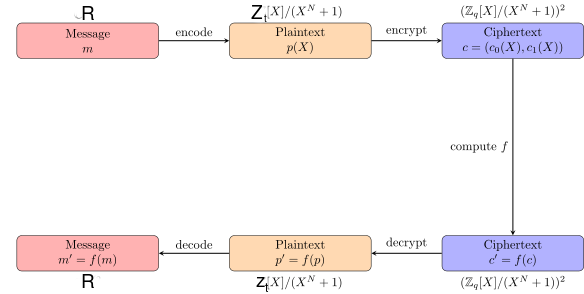
\includegraphics[width=0.85\textwidth]{bfv-diagram.png}
\end{figure}


\end{frame}
%%%%%%%%%%%%%%%%%%%%%%%%%%%%%%%%%%%%%%%%%%%%%%%%%%%%%%%%%%%%%%%%%%%%%%%%%%%%%%%%%%%%%%%%%%%%%%%%%%%%

% combinarla con la de los parametros.
\begin{frame}[noframenumbering]

\frametitle{Parameters}

The parameters depends in the security level needed and amount of operations that will made.

\vspace{-0.2cm}

Some usual parameters to get the sense of what we are doing:
\vspace{-0.2cm}

$N$ = 8192, 16384, 32768 $\rightarrow$ bigger $N$ $\approx$ bigger noise budget but bigger ciphertex and heavier computation.
\vspace{-0.2cm}

    $q$ = $2^{218}$,   $2^{438}$,  $2^{881}$ $\rightarrow$ bigger $q$ $\approx$ bigger noise budget but bigger ciphertex and heavier computation.
\vspace{-0.2cm}

    $t$  << $q$. $\rightarrow$ smaller $t$ $\approx$ bigger noise budget but less precision.

\vspace{-0.2cm}
    $k\in [3,5], 9, 16 \rightarrow$ generally select to stay in 64bits arithmetic's, bigger parameters, bigger $k$.
% que significa q/t


\vspace{-0.2cm}
    RNS example: $k$=3, $x=123456789$, $M = 17 * 257 * 65537$ (3 coprimes of q).

\vspace{-0.2cm}
    $x_{RNS} = [x$ $mod$ $17,$ $x$ $mod$ $257,$ $x$ mod $ 65537] = [1, 157, 50618]$ CRT to come back
\end{frame}

\begin{frame}[noframenumbering]

    \frametitle{Encryption}

    Encryption has two phases:

    - From an integer m to plaintext M $\rightarrow$ Easy, one way: binary representation as Polynomial coefficient.

    - From plaintext to ciphertext using $PK = (PK_1, PK_2)$:

    \begin{itemize}
        \item Sample a polynomial $u$ from $\mathcal{R}_2$.
        \item Sample polynomial errors $e_1$ and $e_2$ form a Gaussian distribution.
        \item Calculate scaling factor $\triangle = \lfloor q/t\rfloor $
        \item Encryption of plaintext M is $C=(C_1, C_2)$
    \end{itemize}
    %
    \begin{align}
        &C_1 = [PK_1 * u + e_1 + \triangle M ]_q\nonumber \\
        &C_2 = [PK_2 * u + e_2]_q\nonumber
    \end{align}


\end{frame}
%%%%%%%%%%%%%%%%%%%%%%%%%%%%%%%%%%%%%%%%%%%%%%%%%%%%%%%%%%%%%%%%%%%%%%%%%%%%%%%%%%%%%%%%%%%%%%%%%%%%


\begin{frame}[noframenumbering]

    \frametitle{Multiplication}

    High computational cost:
    \vspace{-0.15cm}

    $C_{mul} = C*C' = (C_1*C_1',C_1*C_2'+C_2*C_1', C_2*C_2') = (C_a,C_b,C_c)$
    \vspace{-0.15cm}

    \textbf{Problem}: If we keep multiplying, the number of Polynomials will grow and will be needed
    the squared of the SK.

    \textbf{Relinerize}:
    $EvalK = (-PK_1+SK^2, PK_2)$

    $C_{mul} = (C_a, C_b, C_c)\approx ([C_a+EvalK_1*C_c]_q, [C_b+EvalK_2*C_c]_q)$

    \textbf{Other problem}: high noise growth: we are multiplying the errors of the two ciphertexts, the result error
    grows a lot!
    \vspace{-0.1cm}

    \textbf{Solution}: \vspace{-0.3cm}
    \begin{itemize} \vspace{-0.2cm}
        \item Select the lowest parameters for the ''exact'' amount  of operations needed (HE). \vspace{-0.2cm}
            \vspace{-0.25cm}
        \item Use Bootstrapping  (FHE). Even more demanding (multiple multiplications like $C_{mul}$).
    \end{itemize}
\end{frame}
%%%%%%%%%%%%%%%%%%%%%%%%%%%%%%%%%%%%%%%%%%%%%%%%%%%%%%%%%%%%%%%%%%%%%%%%%%%%%%%%%%%%%%%%%%%%%%%%%%%%

\begin{frame}[noframenumbering]
\frametitle{}
\begin{figure}
    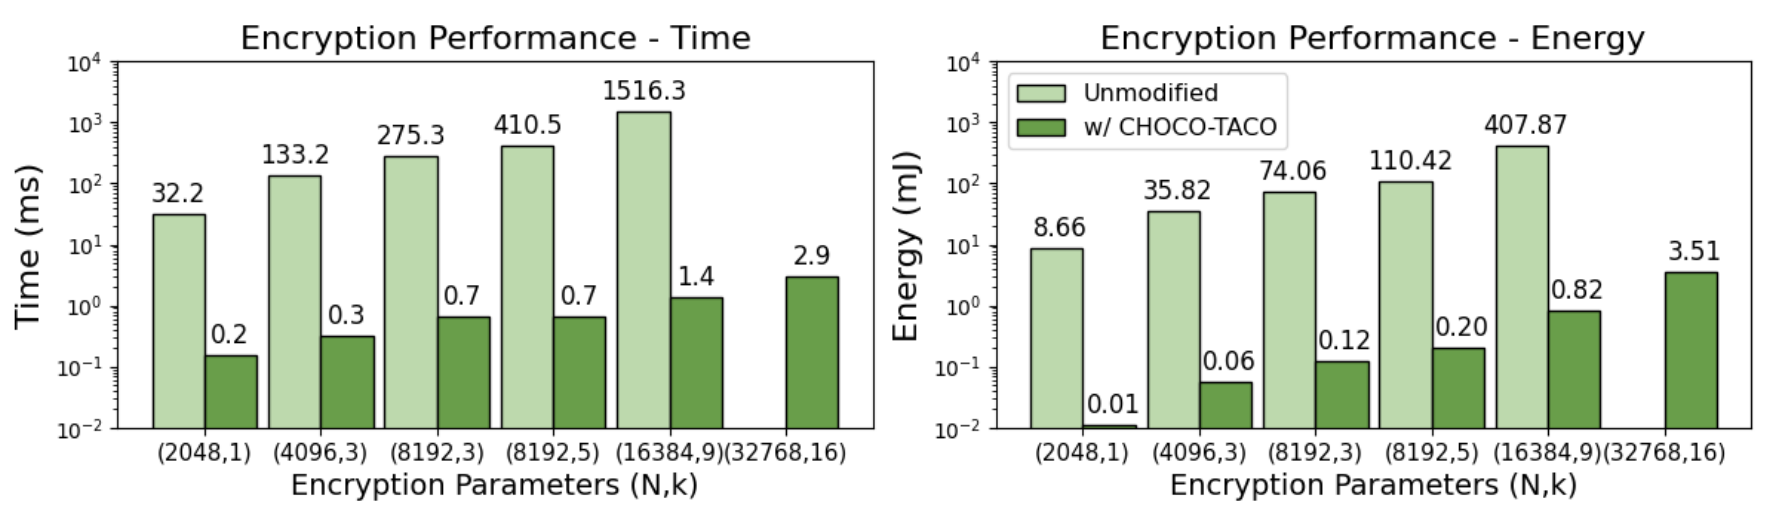
\includegraphics[width=0.85\textwidth]{SW_comp.png}
\end{figure}

\end{frame}
%%%%%%%%%%%%%%%%%%%%%%%%%%%%%%%%%%%%%%%%%%%%%%%%%%%%%%%%%%%%%%%%%%%%%%%%%%%%%%%%%%%%%%%%%%%%%%%%%%%%

\begin{frame}[noframenumbering]
\frametitle{}
\begin{figure}
    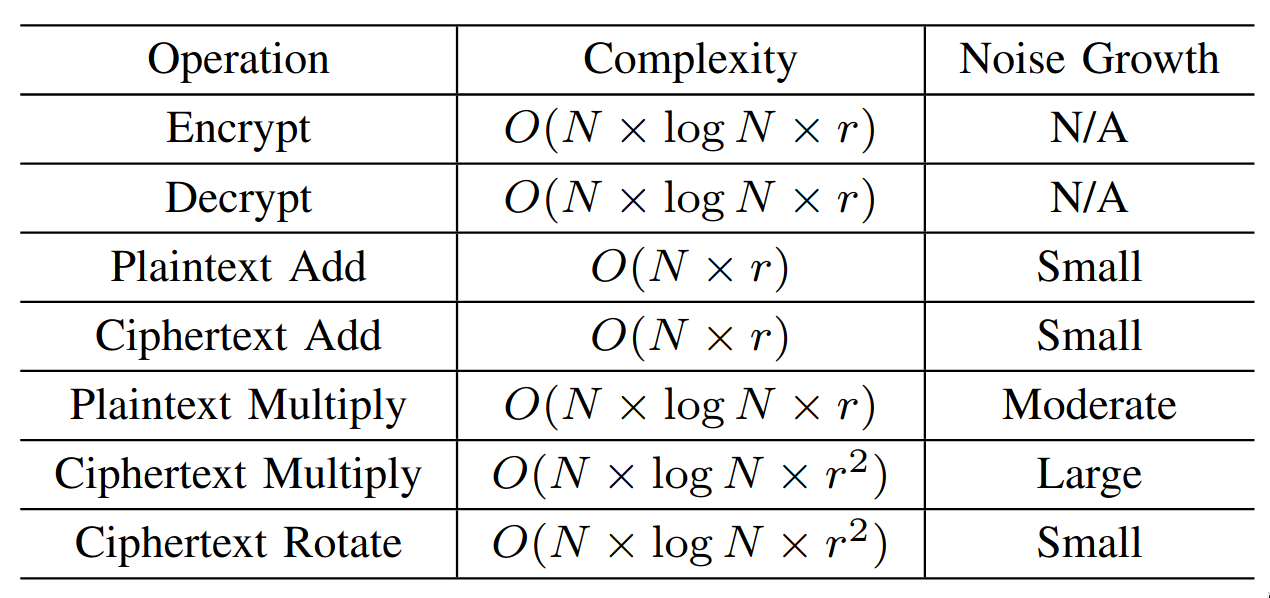
\includegraphics[width=0.75\textwidth]{complexity.png}
\end{figure}

\end{frame}
%%%%%%%%%%%%%%%%%%%%%%%%%%%%%%%%%%%%%%%%%%%%%%%%%%%%%%%%%%%%%%%%%%%%%%%%%%%%%%%%%%%%%%%%%%%%%%%%%%%%

\begin{frame}[noframenumbering]
\frametitle{}
    Pseudo-Random Number Generation: implements Blake3 cryptographic hash (SEAL uses Blake2).
    565 MB/s of random values at peak and 201 MB/s on average.

    Polynomial Multiplication: Iterative NTT and INTT modules. pipeline, SIMD memory acces, following a
    butterfly dataflow pattern.

    Addition and modulus Switching: coefficient-wise addition, passing results to the modulus Switching module.

    Message Encoding: pair of small NTT and INTT blocks. Converts in k-1 RNS residues.

    Memory: each modules has embedded SRAM. Empirically sub-1kb. NTT and INTT operate on a fully
    polynomial $\rightarrow$ 64kB with N=8192 and k=3.

    Parallelism: TACO exploits pipelining and data parallelismo of independent RNS residues and coefficients.


\end{frame}
%%%%%%%%%%%%%%%%%%%%%%%%%%%%%%%%%%%%%%%%%%%%%%%%%%%%%%%%%%%%%%%%%%%%%%%%%%%%%%%%%%%%%%%%%%%%%%%%%%%%


\begin{frame}[noframenumbering]

\frametitle{CHOCO-TACO}
% Entender las flechas de colores y como se hace cob RNS.
% entender el mod switching de ahi.
    \vspace{-0.5cm}
\begin{equation*}
    Enc([P_0,P_1],m) = ([\triangle m + P_0u+e_1]_q, [P_1u+e_2]_q)
\end{equation*}
\pause
    \vspace{-1.cm}
\begin{figure}
    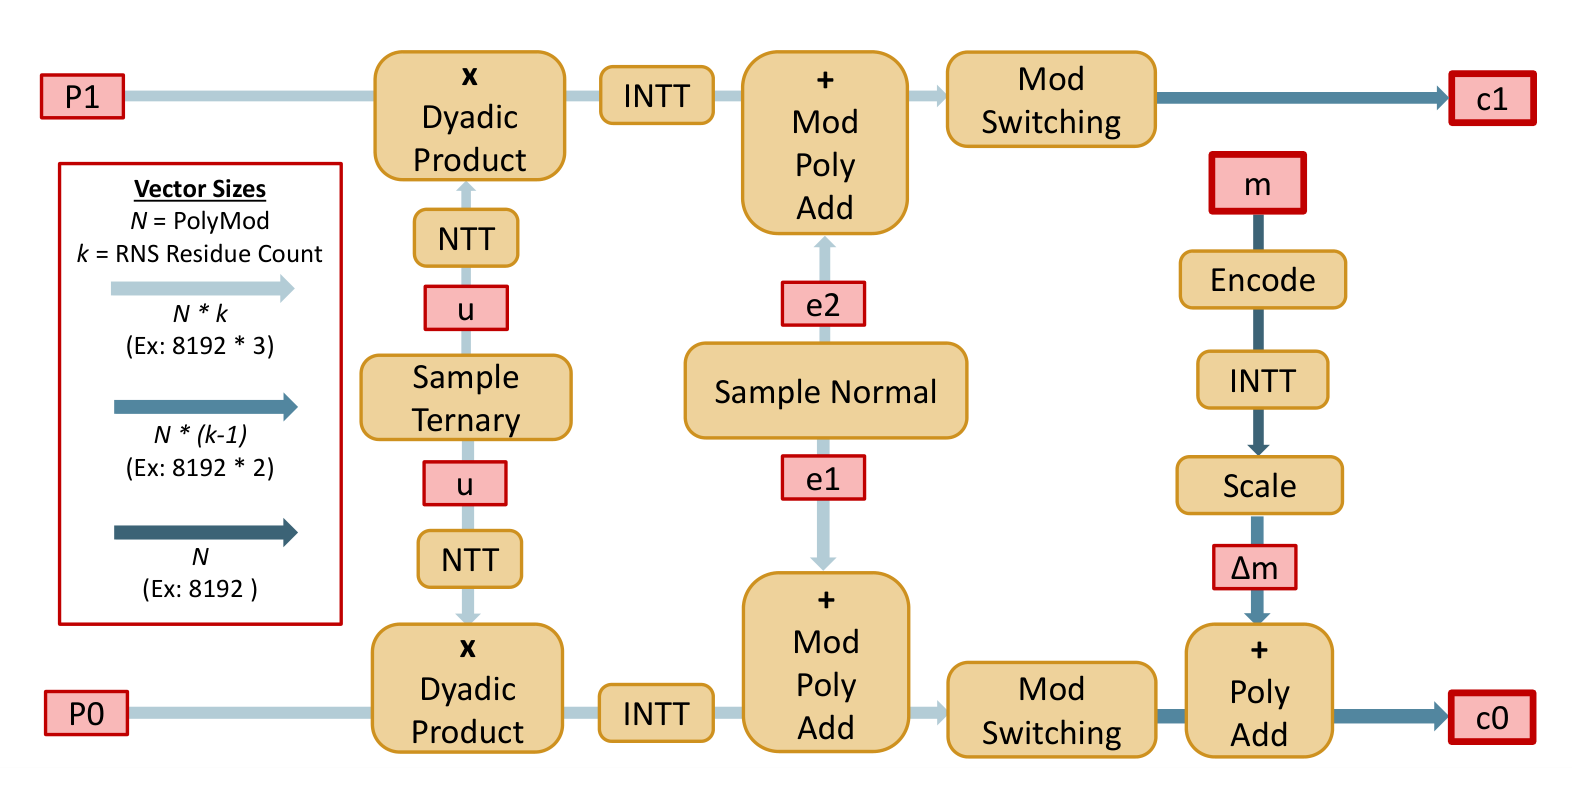
\includegraphics[width=0.95\textwidth]{pipeline.png}
\end{figure}
    \vspace{-0.5cm}

Decryption is similiar. Less parallelism, only 125x time
%\begin{equation*}
%    Dec(SK,[c_0,c_1]) = [\lfloor \frac{t}{q}[c_0+c_1SK]_q\rfloor]_t
%\end{equation*}


% Modulus Switching

% al multiplicar dos polynomios en el espacio NTT es simplemente elemento a elemento C[i] = A[i]*B[i]. y despues
% transformamos de nuevo con INTT

\end{frame}
%%%%%%%%%%%%%%%%%%%%%%%%%%%%%%%%%%%%%%%%%%%%%%%%%%%%%%%%%%%%%%%%%%%%%%%%%%%%%%%%%%%%%%%%%%%%%%%%%%%%

\begin{frame}[noframenumbering]
\frametitle{}
\begin{figure}
    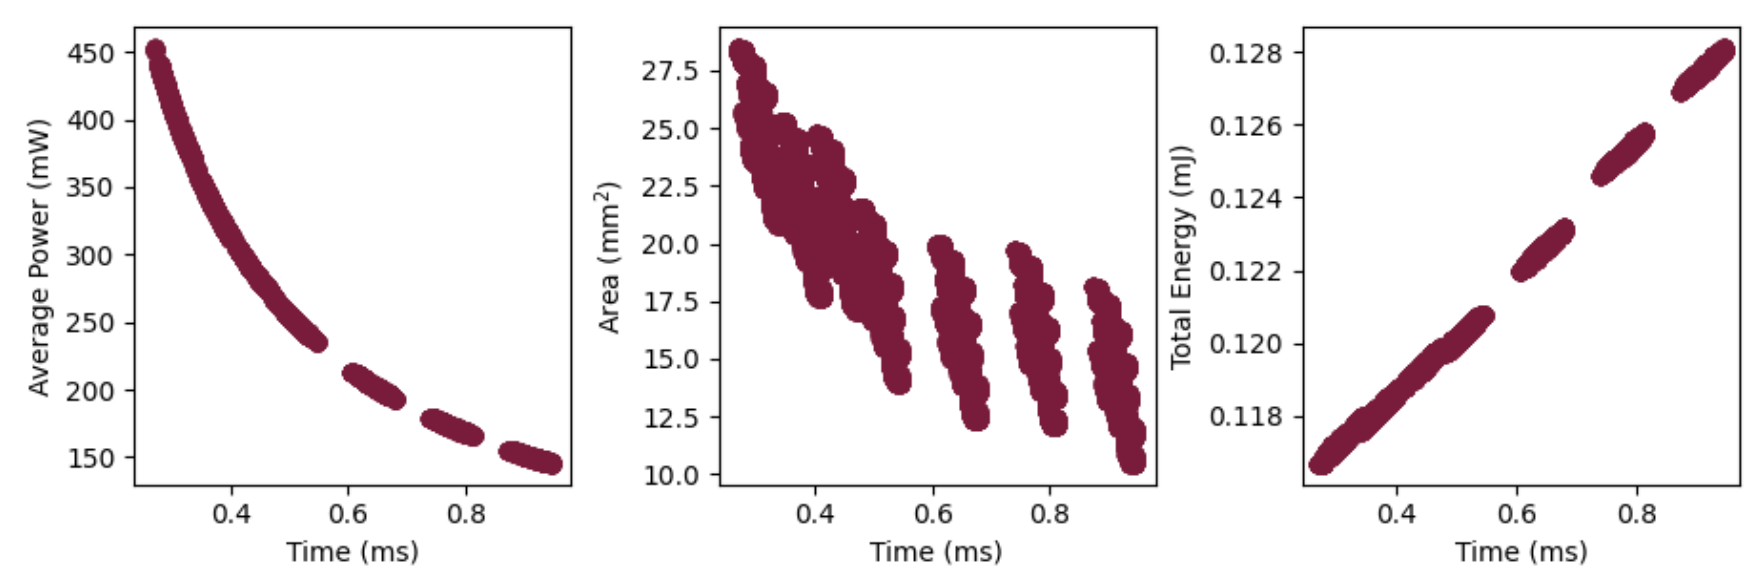
\includegraphics[width=0.85\textwidth]{design-space.png}
\end{figure}
\end{frame}
%%%%%%%%%%%%%%%%%%%%%%%%%%%%%%%%%%%%%%%%%%%%%%%%%%%%%%%%%%%%%%%%%%%%%%%%%%%%%%%%%%%%%%%%%%%%%%%%%%%%
\end{document}
